\section{OO}
\subsection{Type Descriptors}
Type Descriptors are used in Runtime System and can used for type checking and type safety. It's also usable for ancestor table for fast type tests/casts and the virtual table to dispatch cirtual methods.

\begin{lstlisting}
A x;
x = new C();
if (x instanceof B) { }
\end{lstlisting}

\begin{enumerate}[nosep]
	\item Dereference object in heap (via x)
	\item  Dereference type tag in block $=>$ leads to class descriptor of C
	\item Look up slot 1 (static ancestor level of B) in ancestor table of C descriptor (contains entry B, i.e. pointer to class descriptor of B)
	\item Check if entry is the same as type test operand B $=>$ Yes, i.e. results true
\end{enumerate}

\subsection{Ancestor Table}
\begin{center}
	\includegraphics[width=\columnwidth]{"Images/ancestor table"}
\end{center}

\subsection{Virtaul Table}
\begin{lstlisting}
class A {
  void f() { writeString("1"); }
  void g() { writeString("2"); }
}
class B extends A {
  void h() { writeString("3"); }
  void g() { writeString("4"); }
}
\end{lstlisting}
\begin{center}
	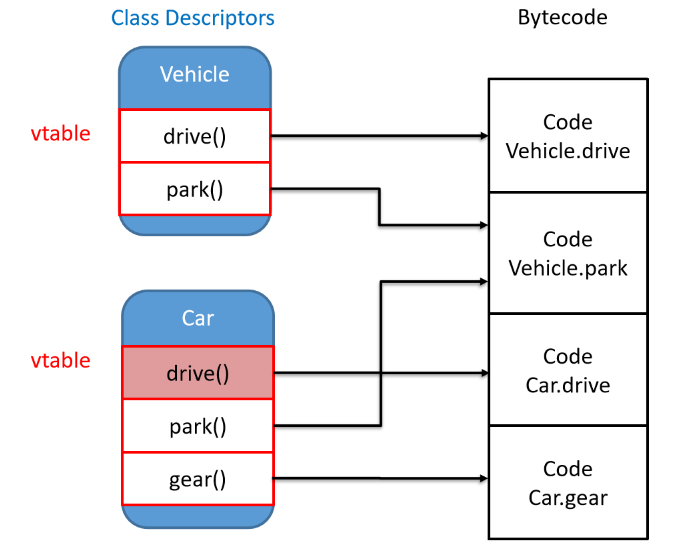
\includegraphics[width=\columnwidth]{Images/vtable}
\end{center}

\begin{enumerate}[nosep]
	\item Dereference object in heap (via x)
	\item Dereference type tag in block $=>$ leads to class descriptor of B
	\item Look up slot 1 (static method position of g()) in virtual table of B descriptor (contains pointer to code B.g())
	\item Branch to the code $=>$ B.g() is called
\end{enumerate}